\chapter{Modeling Approach}
\label{chap:The Model}

\section{Theoretical Framework}
\label{sec:Theoretical_Framework}
We are interested in connecting the interaction rate per unit path length of a photon with energy $E$ to the pair-production cross-section $\sigma_{\text{pair}}(s)$ and the spectral density of background photons $n_{\gamma}(\varepsilon)$. We can do so in the following manner \citep{Kachelrie__2012}
\begin{equation}
    R_{\gamma}(E) = \frac{1}{2}\int_{0}^{\infty}d\varepsilon \,n_{\gamma}(\varepsilon)\int_{-1}^{1}d\mu\,(1-\mu)\,\sigma_{\text{pair}}(s)\,\Theta(s-s_{\min}),
    \label{eq:interaction_rate_first_one}
\end{equation} where $s_{\min}$ is the threshold energy squared for pair production ($s_{\min} = 4m_e^2$ in this case, $m_e$ being the mass of an electron), and $\Theta(s-s_{\min})$ is the Heaviside step function. It is there to ensure we only integrate over energies above the threshold. The pair-production cross-section $\sigma_{\text{pair}}(s)$ is well-known, as one can find in any particle physics textbook. It is given by 

\begin{equation}
    \sigma_{\rm pair}(s)=\frac{3}{4}\,\sigma_{{\rm Th}}\, \frac{m_e^2}{s}
     \left[(3-\beta^{4})\ln\frac{1+\beta}{1-\beta}-2\beta(2-\beta^{2})\right]\!,
    \label{eq:sigma-pair}
\end{equation} where $\sigma_{\rm Th}$ is the Thomson cross-section, $\beta \equiv \sqrt{1-4\,m_e^2/s}$, $s = 2E\varepsilon\,(1-\mu)$ and $\mu \equiv \cos(\theta)$, where $\theta$ is the angle between the incident high-energy photon ($E$) and the background photon ($\varepsilon$).

From equation \eqref{eq:interaction_rate_first_one}, it is convenient to rewrite the integrals in terms of the mandelstam variable $s$, and swap the order of integration. Doing so, we get the following:

\begin{equation*}
    R_{\gamma}(E) = \frac{1}{8E^2}\int_{0}^{\infty}\frac{d\varepsilon}{\varepsilon^2}\,n_{\gamma}(\varepsilon)\int_{s_{\min}}^{4E\varepsilon}ds\,s\,\sigma_{\text{pair}}(s) =
    \label{eq:interaction_rate_second_one}
\end{equation*}

\begin{equation}
    =  \frac{1}{8E^2}\int_{4m_ec^2}^{4E\varepsilon_{\max}}ds\,s\,\sigma_{\text{pair}}(s)\int_{\frac{s}{4E}}^{\varepsilon_{\max}}\frac{d\varepsilon}{\varepsilon^2}\,n_{\gamma}(\varepsilon)
    \label{eq:interaction_rate_third_one}
\end{equation}
Notice that for a given s, we have $s \leq 4E\varepsilon$, which implies that $\varepsilon \geq \frac{s}{4E}$. This is the reason for the lower limit of the $\varepsilon$ integral. The upper limit of the $\varepsilon$ integral is $\varepsilon_{\max}$, which is the maximum energy of our background photons.

In order to find this interaction rate of photons with energy $E$, we need to know the spectral density of background photons $n_{\gamma}(\varepsilon)$. To derive this quantity, we first need to know what the spectral energy distribution of background photons looks like. \citet{Eichmann_2022} derived in their work a spectrum of background photons for the starburst and X-ray corona region. This background spectrum will be used to model the density of background photons $n_{\gamma}(\varepsilon)$ inside the AGN's corona:


\begin{figure}[H]
    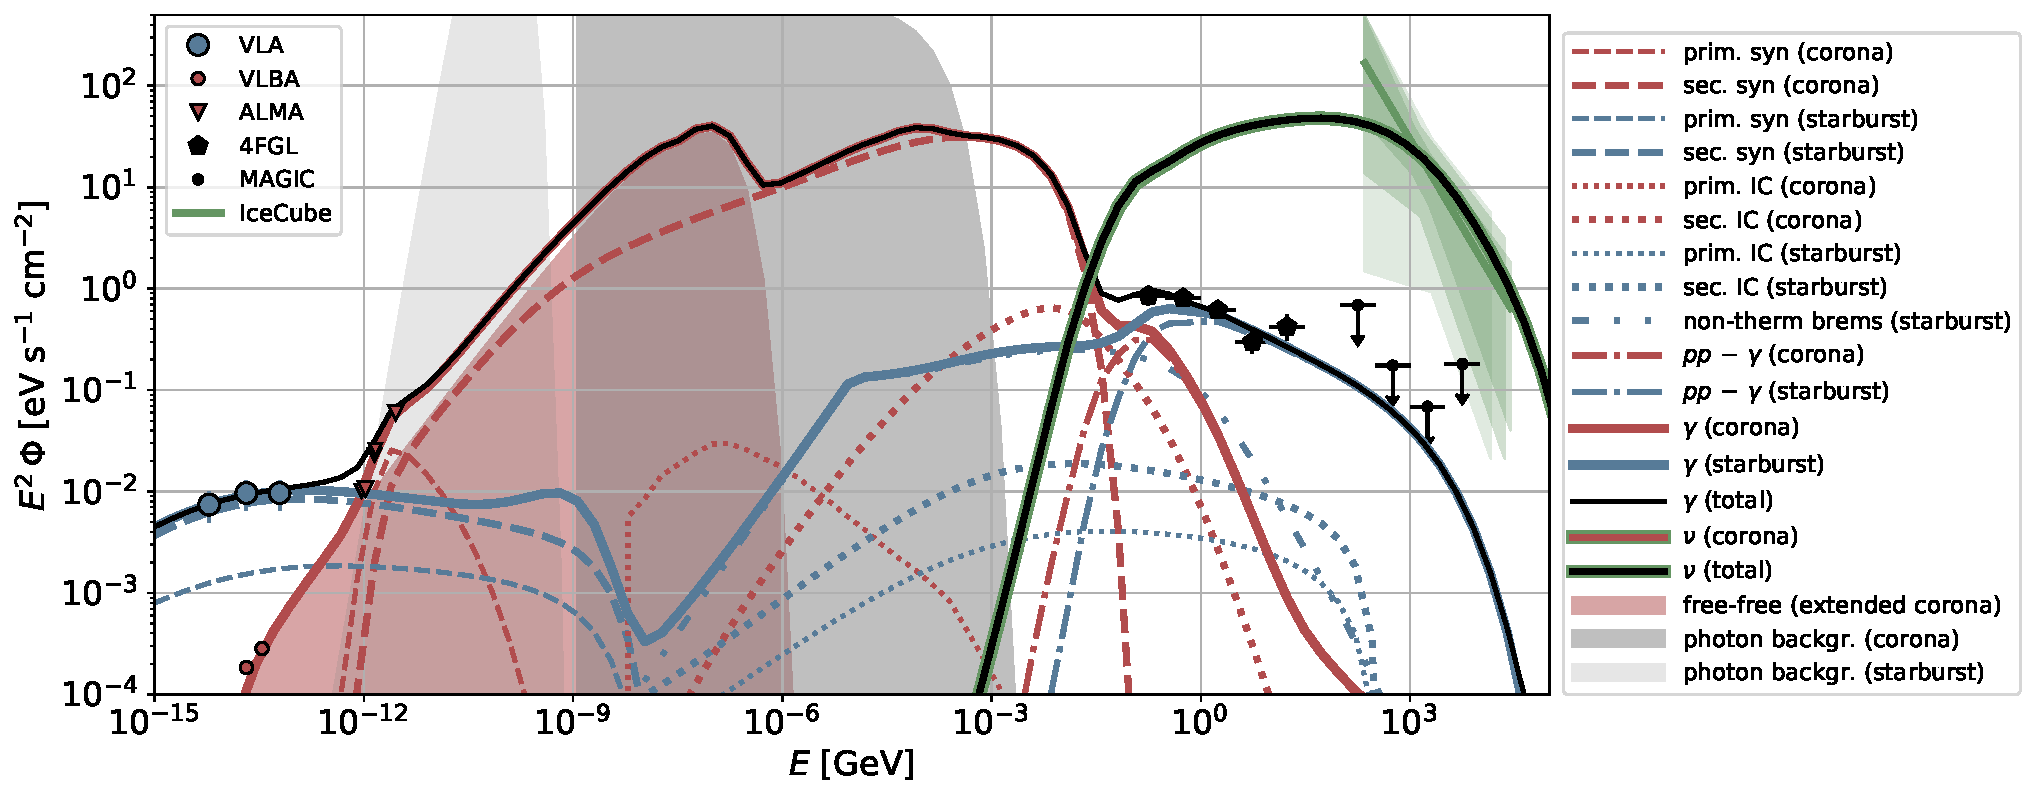
\includegraphics[width=\textwidth]{Figures/fit5b2_SED_details.pdf}
    \centering
    \caption{The model predictions of the \emph{photon and neutrino} SED of NGC\,1068 with respect to the data---red markers refer to a beam size of $\sim (0.02-0.06)\,\text{arcsec}$, and black or blue markers indicate a beam size of $\gtrsim 10\,\text{arcsec}$. The light red area shows the free-free emission from the extended corona. The dark grey area indicates the \emph{internal} flux of the background (target) photon fields (disk- and torus emission as well as Comptonized X-rays of the AGN's corona) of the central AGN and the light grey area indicates the thermal IR emission by dust grains of the starburst region. Note that the torus attenuation is not taken into account here. Figure taken from \citet{Eichmann_2022}.} 
    \label{fig:background_spectral_density}
\end{figure}

The red line marked as $\gamma \text{ (corona)}$ in the legend of the figure above will be used to model the spectral density of background photons $n_{\gamma}(\varepsilon)$\footnote{It is important to note the circular reasoning here. Ideally, the cascaded spectrum should be used to simulate the cascading of the same particles. However, for simplicity, I will assume the aforementioned to be the pre-existing spectrum within the corona.}.

$n_{\gamma}(\varepsilon)$ can be connected to $\Phi(\varepsilon)$ in the following manner: we know that the differential flux of background photons relates to the specific intensity $I(\varepsilon)$ by

\begin{equation}
    \Phi = \int d\Omega I \cos \vartheta.
    \label{eq:flux_specific_intensity}
\end{equation}

For a spherical source of radius $R$ at a distance $d$, $\Omega = \pi \left(\frac{R}{d}\right)^2$

We can also connect $I(\varepsilon)$ to the spectral density of background photons $n_{\gamma}(\varepsilon)$ using

\begin{equation}
    n_{\gamma}(\varepsilon) = \frac{4\pi}{c}I(\varepsilon),
    \label{eq:n_phi}
\end{equation} where $c$ is the speed of light. By combining equations \eqref{eq:flux_specific_intensity} and \eqref{eq:n_phi}, we can find the spectral density of background photons $n_{\gamma}(\varepsilon)$ in terms of $\Phi(\varepsilon)$
\begin{equation}
    n_{\gamma}(\varepsilon) = \frac{4}{c}\left(\frac{d}{R_c}\right)^2\Phi(\varepsilon),
    \label{eq:n_gamma}
\end{equation}
where $d$ is the distance to the AGN, and $R_c$ is the radius of the corona.

For this work, the distance to NGC1068 is assumed to be $d = 10.1$ Mpc. This value comes from \citet{padovani2024highenergyneutrinosvicinitysupermassive}. The coronal radius can be parametrized as $R_c = \eta R_s$, with $\eta \sim 10 - 100$, and $R_s$ being the Schwarzschild radius of the black hole, calculated\footnote{Assuming a non-rotating Schwarzschild black hole with mass $M = 1.3 \times 10^7 M_{\odot}$ \citep{Blackhole}} to be around $1.4 \times 10^{-6}$ pc.

A useful quantity to calculate is the optical depth of the corona. This relates to the probability of a photon with a certain energy interacting trough pair production. The optical depth $\tau_{\gamma\gamma}$ is given by 
\begin{equation*}
    \tau_{\gamma\gamma} = R_{\gamma} \cdot  R_c.
\end{equation*}

Figure \Ref{fig:optical_depth_as_function_of_corona_radius} shows the optical depth of the corona as a function of the energy of the photons for different values of $R_c$.

\begin{figure}[ht]
    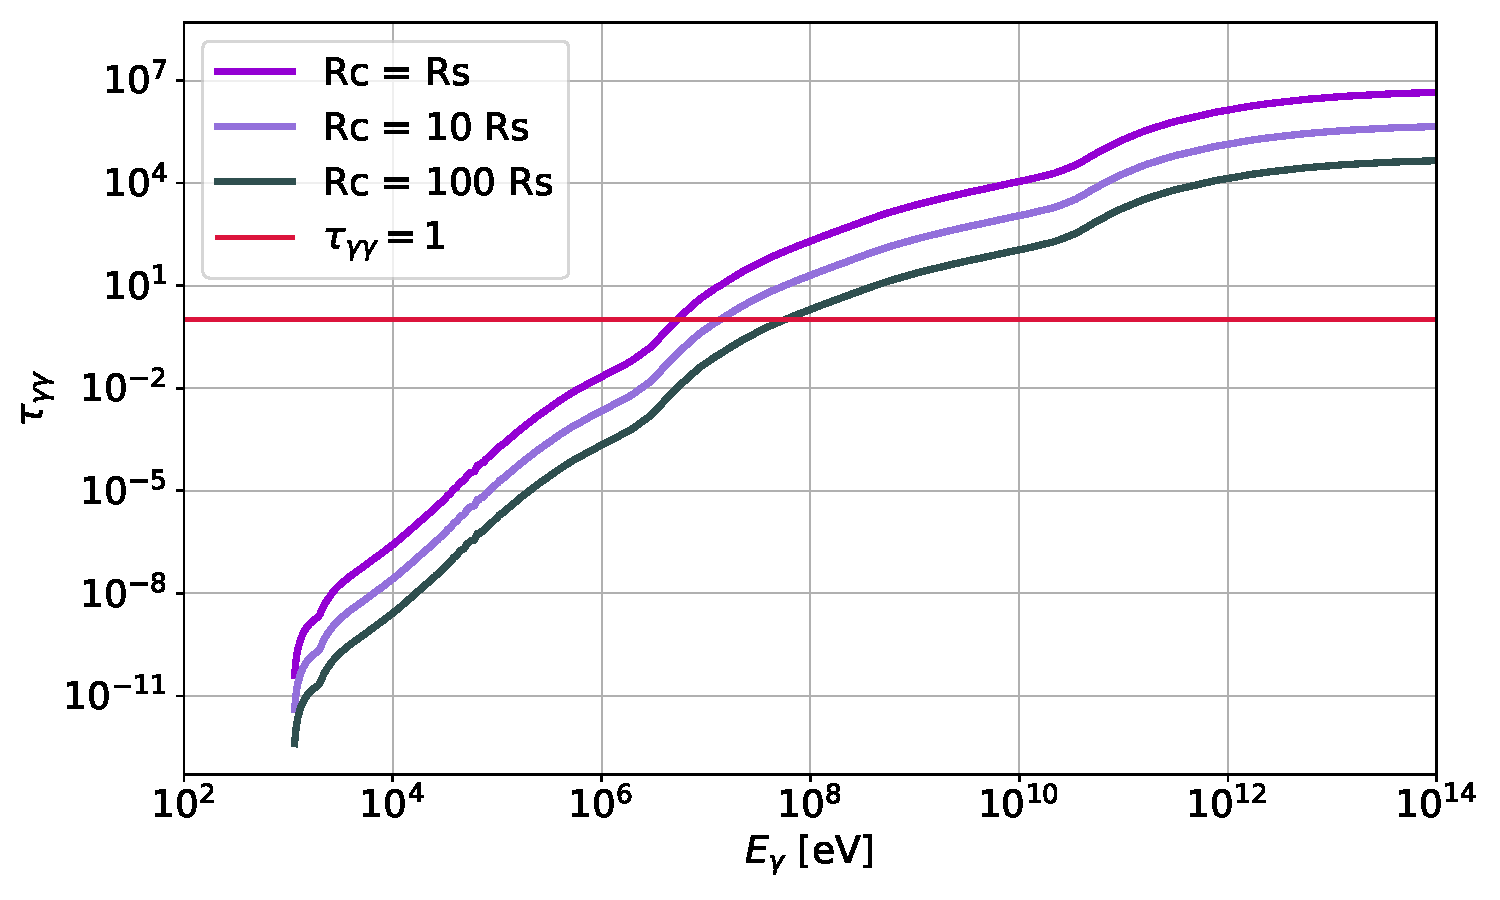
\includegraphics[width=0.8\textwidth]{Figures/OpticalDepths.pdf}
    \centering
    \caption{Optical depth of NGC1068's corona as a function of the energy of the photons, represented for different values of the corona radius. One can see that the corona is optically thick for high-energy photons ($\tau_{\gamma\gamma}>1$), and optically thin for low-energy photons ($\tau_{\gamma\gamma}<1$), meaning that high-energy photons are prone to interacting with the corona more than low-energy ones.}
    \label{fig:optical_depth_as_function_of_corona_radius}
\end{figure}


\section{Implementation}

The implementation of this model was performed in MATLAB. The code is available in Appendix A, and it is structured in the following way:

\begin{itemize}
    \item Initialization: Defines physical constants and loads observational data (e.g., from Fermi-LAT, IceCube) used for comparison. However, as we want to test the model for different values of certain parameters, these don't get defined here.
    \item Parameter Loops: Nested loops iterate over the model parameters being tested, such as the coronal radius ($R_c$), the initial radial distribution parameter ($\alpha$, see Eq. \ref{eq:alpha}), and the maximum turning angle ($\theta_{\max}$).
    \item Interaction Rate Calculation: within the loops, the code calculates the interaction rate per unit length, $R_{\gamma}(E)$, using the theoretical framework (Section \ref{sec:Theoretical_Framework}) for the current value of $R_c$. These values are stored in a matrix, as a function of the energy of the photons.
    \item Cascade simulation: Finally, the code calculates the cascading of photons in the corona, and stores the results for the parameters defined. It is assumed that the photons produced in the corona have the same energy distribution as that of the neutrinos we receive. 
    This part is very intricate, and has different steps to it, which are detailed in Section \ref{sec:RandomWalk}.
\end{itemize}

\section{Simulation of Cascading via Random Walk}
\label{sec:RandomWalk}

There are several parameters which affect the cascading of photons in the corona. These include the coronal radius, the maximum turning angle of the particles and the alpha value, which controls the initial distribution of photons. The random walk is a stochastic process, and as such, it is important to consider the different sources of error one can encounter when developing these kinds of models, such as the number of particles simulated or the binning of the energy spectrum. The code is structured in a way that allows for easy modification of these parameters, so that one can test different values and see how they affect the results.

For each energy bin, a number of particles which is proportional to the flux at said energy is chosen to simulate. The particles are chosen according to the formula
\begin{equation}
    \#_{\text{part., } E}=\left\lfloor \rho \frac{\Phi_E \Delta_E}{\min(\Phi_E \Delta_E)} \right\rceil,
\end{equation}
$\Phi_E$ and $\Delta_E$ being the flux and bin width as a function of the energy. The latter of the two can be increased to reduce statistical noise. The numerator is divided by its minimum to ensure normalization: this way we make sure we simulate at the very least one particle for the lowest flux. Finally, $\rho$ is a multiplicative factor, which can be changed to modify the overall number of particles we want to simulate. The program then rounds the resulting value to the nearest integer, giving the number of particles for each energy bin.

For each particle:
\begin{enumerate}
\item The initial position is randomly placed inside the corona using a power law of the shape
\begin{equation}
r = R_c \cdot \text{rand}^{(1/\alpha)}.
\label{eq:alpha}
\end{equation}
\begin{figure}[ht]
    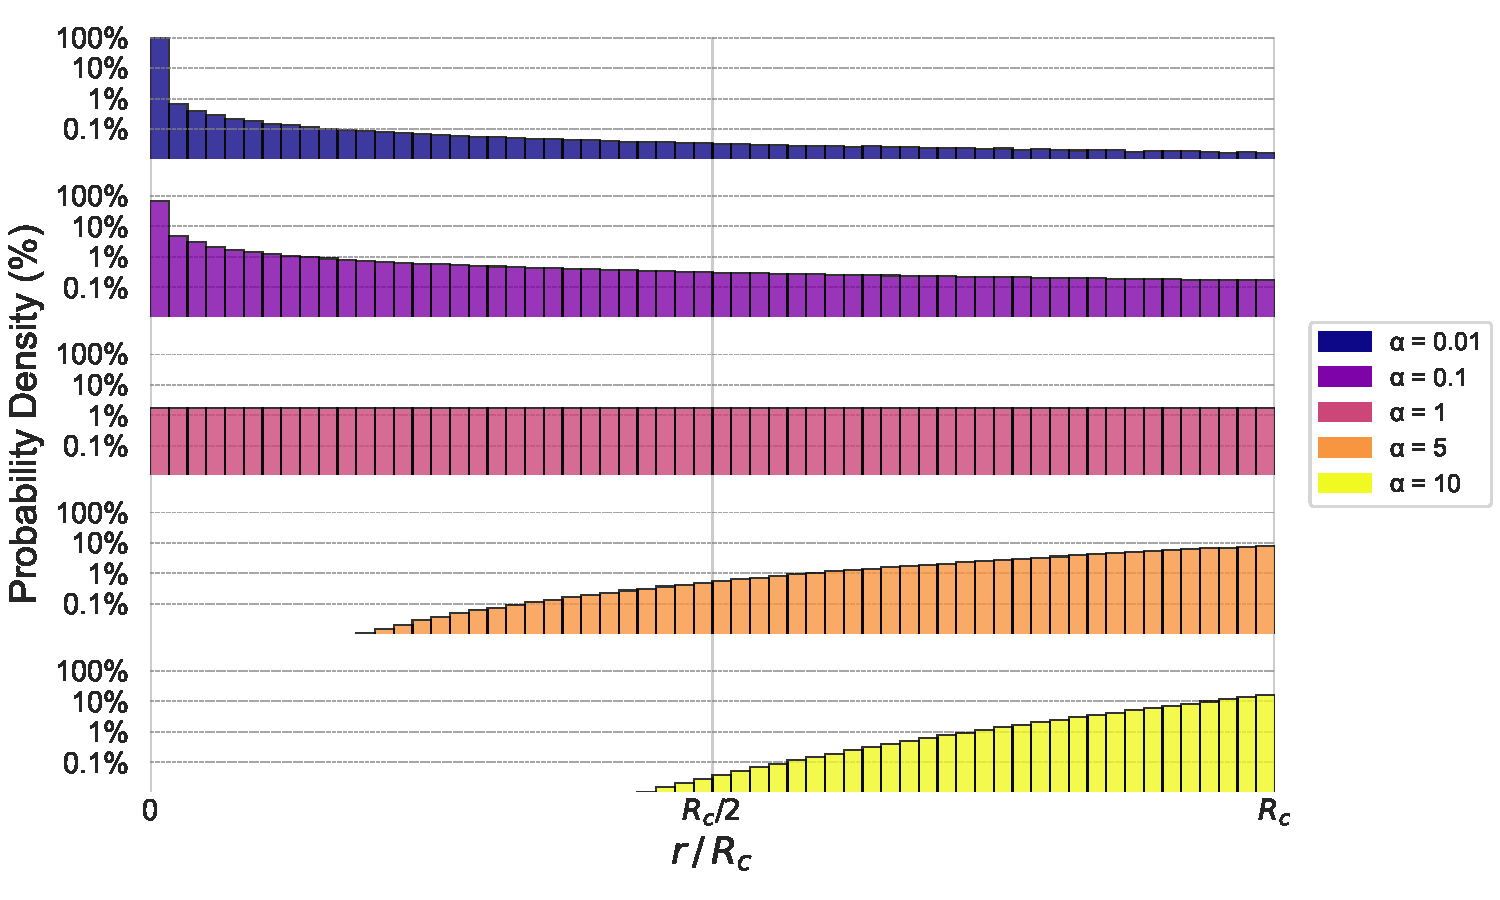
\includegraphics[width=\textwidth]{Figures/InitialDistributions.pdf}
    \centering
    \caption{Initial distributions of the photons for different values of $\alpha$. The y-axis shows the percentage of photons, and the x-axis shows the distance from the center of the corona. In order to account for the division by zero in the case of $\alpha=0$, the program assumes all particles start at the origin in this case.}
    \label{fig:initial_distributions}
\end{figure}

\item Each particle is assigned a random initial direction, uniformly distributed on a sphere.
\item The particle propagates until it exits the corona. Each step it takes has a length determined by
\begin{equation}
L = -\frac{\ln (\text{rand})}{R},
\end{equation}
where $R$ is the interaction rate previously calculated as a function of the energy of the photon.
\item After each collision, the particle's direction is updated. The new direction is determined by a random angle $\theta$ sampled from a uniform distribution between $-\theta_{\max}$ and $\theta_{\max}$\footnote{This is a simplification of the actual process. In reality, in order to achieve truly random directions (not biased towards the poles), the program generates uniformly distributed points on a spherical cap of max angle $\theta_{\max}$ around the z axis, which is then rotated to the previous direction. The random point selected becomes the new direction of the particle. The Manim folder inside the GitHub repository contains a visualization of this process.}.

\item The particle's energy is multiplied by a random fraction sampled from a predefined probability distribution\footnote{It must be noted that the process being modeled here omits the production of $e^+e^-$ pairs, assuming they recombine quickly into  gamma rays. Hence, the true physical process being modeled here is scattering of gamma rays, and not cascading.}. The probability distribution is defined in the code, and can be changed to test different distributions. The default one is a Gaussian distribution with a mean of 0.5 and a standard deviation of 0.01. This essentially means that the energy of the particle is multiplied by a random value between 0.49 and 0.51.\footnote{Here, another simplification is made. When two photons produce a pair and $E\varepsilon/m_e^2c^4\gg1$, the fraction of energy lost is $f\approx [\ln(2E\varepsilon/m_e^2c^4)]^{-1}$. However, if $E\varepsilon/m_e^2c^4\sim 1$, $f=0.5$. Thus, it is assumed that $\varepsilon \sim m_e^2c^4/E$. \citep{energyfraction}}
\item In order to account for the energy lost in the process, which is transferred to the background photons, the program assumes that in every step a new particle is created with the exact same energy as the original photon, which cascades in the same way. Meaning we end up with $2^N$ particles with the same energy, $N$ being the number of collisions in the cascade\footnote{This is another approximation. In reality, one should consider the full cascade of each newly produced particle individually. However, this would increase computational costs exponentially.}.
\item Finally, in order to determine the flux as a function of the energy (proportional to the number of particles), the particles are binned logarithmically with spacing which is also specified in the program ($\Delta_E$), and can be changed to reduce statistical noise, in turn reducing the need for computing a high number of particles.
 
\end{enumerate}



% \chapter{Theory}
% \label{chap:Theory}

% The theory section is not as common to include as the other sections included in this document. Some work is theory-heavy, and it can be beneficial to split the theory part from the background and methodology parts of the document. In this document, we will rather use this section to show some important \LaTeX commands that you are likely to use.

% When you write in \LaTeX, try to just follow the given style. You might not like the exact way of the given style in your document, but if you try to change it with small commands everywhere, you will probably end up with a document that looks worse, and you will spend a lot of time writing \LaTeX code in your document.

% \section{Equations}

% A simple equation or variable can be written within sentences using the dollar sign on each side, for example, writing \verb=$a$= will show up as $a$. The usual way of including an equation on a separate line is either by using double dollar signs, such as this:
% $$E = mc^2$$
% or using the \texttt{equation} environment:
% \begin{equation}
%     E=mc^2
%     \label{eq:Einstein}
% \end{equation}
% \sloppy Note that the \texttt{equation} environment will enumerate the equation, and allow you to add a label that you can refer to later. When labeling the equations, you can refer to them using \verb=\eqref{<label>}=, which will give you an equation reference like Eq.~\eqref{eq:Einstein}.

% The text below shows an example of how to align equations on the equal sign, with only one reference for both. This may be useful for when they are linked and are actually only one equation but splitting them up makes it more readable.
% \begin{equation}
% \begin{aligned}
%         a &= \sin^{2}(\Delta\phi/2) + a \sin^{2}(\Delta\phi/2) \\
%          &= (1+a) \sin^{2}(\Delta\phi/2)
% \end{aligned}
% \label{eq:splitTwoLines}
% \end{equation}
% The whole equation can be referenced as a single equation, Eq.~\eqref{eq:splitTwoLines}. One may also align sub-equations such that they are numbered the same but have a letter differentiating them as shown below\footnote{A footnote explaining something.}. This can be used when they are linked, but you will need to reference both individual parts.

% \begin{subequations}
% \begin{align}
%     \sigma &= \sqrt{\frac{1}{N} \sum_{i=1}^N (x_i - \mu)^2}
%     \label{eq:sd}\\ 
%     \mu &= \frac{1}{N} \sum_{i=1}^N x_i \label{eq:mean}
% \end{align}
% \label{eqn:subeqn}
% \end{subequations}\\
% These equations can be referenced by their specific sub-equation as Eq.~\eqref{eq:sd}, or by the whole group as Eqs.~\eqref{eqn:subeqn}.


% \section{Including figures}

% Figure \ref{fig:qualityDiff} is an example of how to include figures in your \LaTeX document. This is also an example of the difference between a vector-based image format (pdf) and a voxel-based format (png). When possible, always try to use a vector-based image format, as that gives infinite resolution.

% These two figures were created using this simple Python code:

% \lstinputlisting[firstline=1, lastline=17,language=Python]{Figures/createPlot.py}

% So when you create figures using Python, try to save them as pdf, as use the tight boundaries to save some space around the figures.

% \begin{figure}[H]
%   \centering
%   \subfloat[Sinus figure using pdf.]{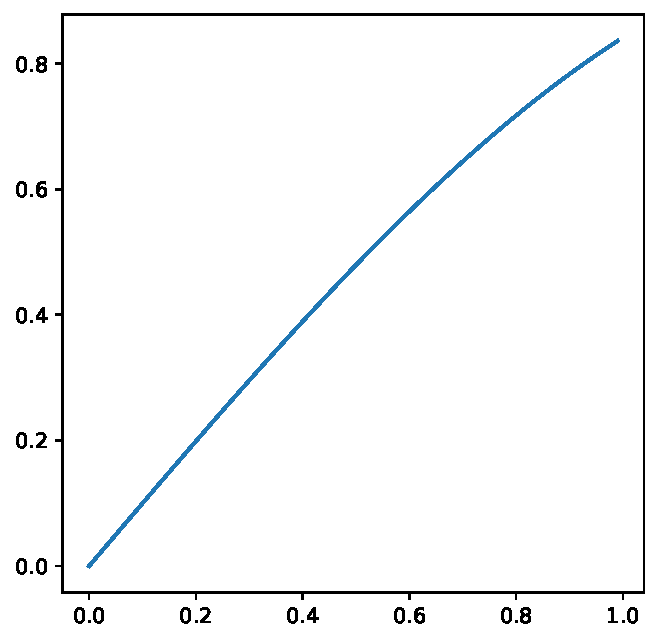
\includegraphics[width=0.45\textwidth]{Figures/sin.pdf}\label{fig:sinpdf}}
%   \quad
%   \subfloat[Sinus figures using png.]{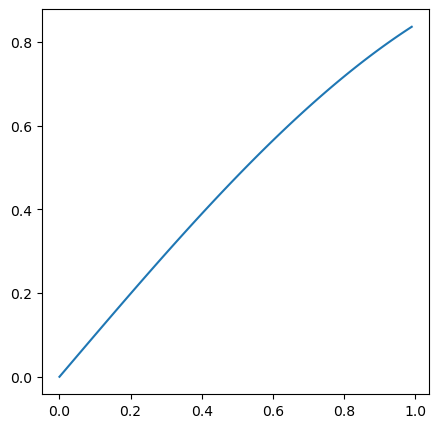
\includegraphics[width=0.45\textwidth]{Figures/sin.png}\label{fig:sinpng}}
%   \caption{Figure (a) shows a pdf figure, while figure (b) shows a png figure. If you zoom in, you will start noticing the difference in quality.}
% \label{fig:qualityDiff}
% \end{figure}

% With Python you could change the size of your figures. This is helpful for getting the right size of text within figures. In Figure \ref{fig:SizeDiff} we compare two different sizes.

% \begin{figure}[H]
%   \centering
%   \subfloat[Sinus figure using size (8,8).]{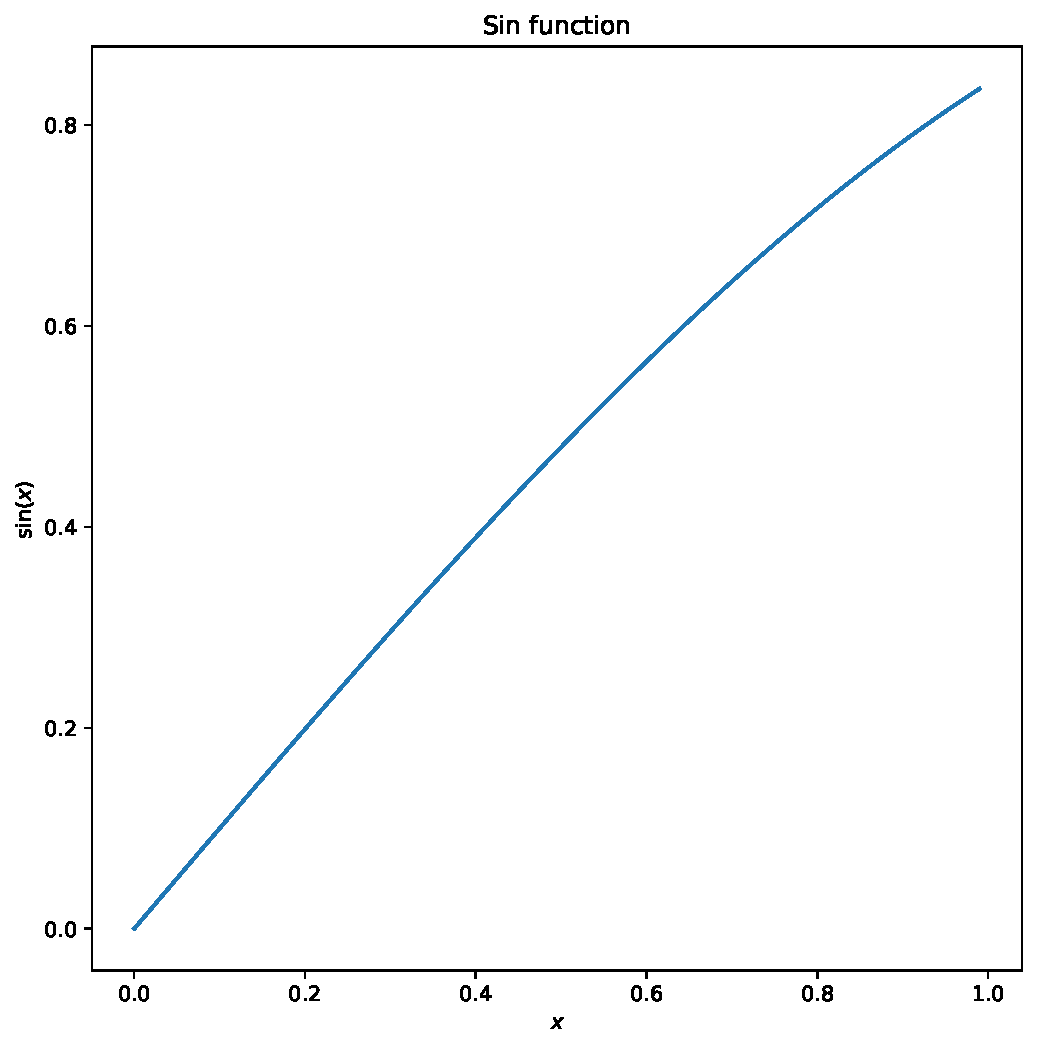
\includegraphics[width=0.45\textwidth]{Figures/sinBig.pdf}\label{fig:sinBig}}
%   \quad
%   \subfloat[Sinus figures using size (4,4).]{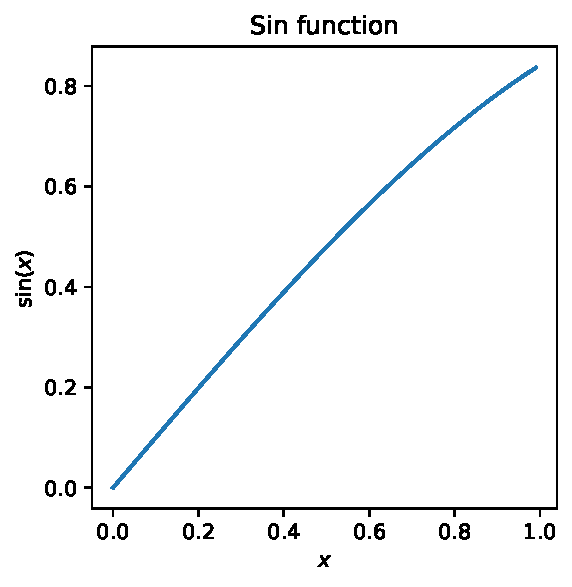
\includegraphics[width=0.45\textwidth]{Figures/sinSmall.pdf}\label{fig:sinSmall}}
%   \caption{This is a comparison between two different figure sizes.}
% \label{fig:SizeDiff}
% \end{figure}


% \section{Chemical notations and units}

% This document has included a package for chemical symbols, \texttt{mchem}. When you write \verb=\ce{CO2}= you will get the chemical notation as \ce{CO2}.

% For units we use the \texttt{siunitx} package. If you write \verb=\SI{10}{\meter\per\second\squared}= you get \SI{10}{\meter\per\second\squared}. The package can be used within math mode (inside the dollar signs). It automatically changes to a fixed notation for numbers, such as \verb=\SI{1E5}{\meter}= gives \SI{1E5}{\meter}.

% \section{Tables}

% Here are two examples of regular tables with data and a table with split headers.

% \begin{table}[ht!]
% \centering
%     \begin{tabular}{ m{3cm} m{2.5cm} m{2.5cm} m{2.5cm} m{2cm} } 
%     \toprule
%     \toprule
%     \textbf{Statistic} & \textbf{Velocity} & \textbf{Altitude} & \textbf{1/Angle} & \textbf{Temp.} \\
%     \midrule
%     Mean    & 122.68    & 240.98   & 93.75     & 13.95 \\[1.3ex]
%     Std     & 224.51    & 145.88   & 60.39     & 4.44  \\[1.3ex]
%     Q1      & 28.00     & 111.60   & 34.15     & 10.60 \\[1.3ex]
%     Median  & 63.00     & 223.20   & 99.59     & 13.30 \\[1.3ex]
%     Q3      & 137.00    & 359.10   & 151.99    & 16.70 \\[1.3ex]
%     Min     & 0.00      & 1.00     & 0.00      & 3.30  \\[1.3ex]
%     Max     & 14519.00  & 616.70   & 180.00    & 32.10 \\[1.3ex]
%     \bottomrule
%     \bottomrule
%     \end{tabular}
% % the square brackets after \caption gives the table a proper title in the list of tables, instead of just inserting the beginning of the table caption
% \caption[Dynamic feature statistics with outliers]{Table of dynamic feature statistics where outliers are included, for all data points. Velocity is given in \textit{m/h}, the altitude in \textit{mamsl}, the inverse trajectory angle in 1/degrees, and temperature in degrees Celsius.}
% \label{table:stat_fliers}
% \end{table}


% \begin{table}[ht!]
% \centering
%     \begin{tabular}{ m{3cm} m{5cm} m{3cm} } 
%     \toprule
%     \toprule
%     \textbf{Area 1} & \textbf{Start date} & \textbf{End date} \\
%     \midrule
%     2018    & 03.06    & 29.06                       \\[1.3ex]
%     2019    & 03.06    & 03.07 or 31.08\footnotemark \\[1.3ex]
%     2020    & 03.06    & 05.09                       \\[1.3ex]
%     \midrule
%     \textbf{Area 2} & \textbf{Start date (farm 1/2)} & \textbf{End date} \\
%     \midrule
%     2012    & 09.06            & 07.09               \\[1.3ex]
%     2013    & 23.06 / 15.06    & 25.08               \\[1.3ex]
%     2014    & 05.06 / 25.06    & 10.09               \\[1.3ex]
%     2015    & 13.06 / 03.07    & 06.09               \\[1.3ex]
%     2016    & 17.06            & 22.07               \\[1.3ex]
%     \bottomrule
%     \bottomrule
%     \end{tabular}
% \caption[Selected time ranges for all data]{Selected time ranges for the data in all areas and all years.}
% \label{table:time_ranges}
% \end{table}

% There are online tools to create \LaTeX tables. This might be a faster way of creating them than writing all the code yourself.
